
\begin{table*}[t]
    \centering
    \caption{Seismicity parameters $b$ and $M_{\max}$ computed for the seismic zones in our region of interest and the reference uniform seismicity model along with the observed maximum magnitude, $M_{\max}^{\mathrm{obs}}$.}
    \begin{tabular}{lccc}
        \cline{2-4}                                                                         \\[-1.6ex]
                        & $b$-value         & $M_{\max}$        & $M_{\max}^{\mathrm{obs}}$ \\[0.6ex]
        \hline                                                                              \\[-1.6ex]
        Azerbaijan      & 1.10 $\pm$ 0.03   & 7.93 $\pm$ 0.34   & 7.7                       \\
        Alborz          & 1.03 $\pm$ 0.03   & 7.85 $\pm$ 0.66   & 7.8                       \\
        Kopeh Dagh      & 0.89 $\pm$ 0.04   & 7.78 $\pm$ 0.31   & 7.6                       \\
        Zagros          & 0.99 $\pm$ 0.02   & 7.47 $\pm$ 0.26   & 7.4                       \\
        Central-East    & 0.95 $\pm$ 0.04   & 7.84 $\pm$ 0.34   & 7.6                       \\
        Uniform Model   & 0.90 $\pm$ 0.02   & 7.87 $\pm$ 0.26   & 7.8                       \\[0.5ex]
        \hline 
    \end{tabular}
    \label{tab:params} 
\end{table*}

\begin{figure*}[t]
    \centering
    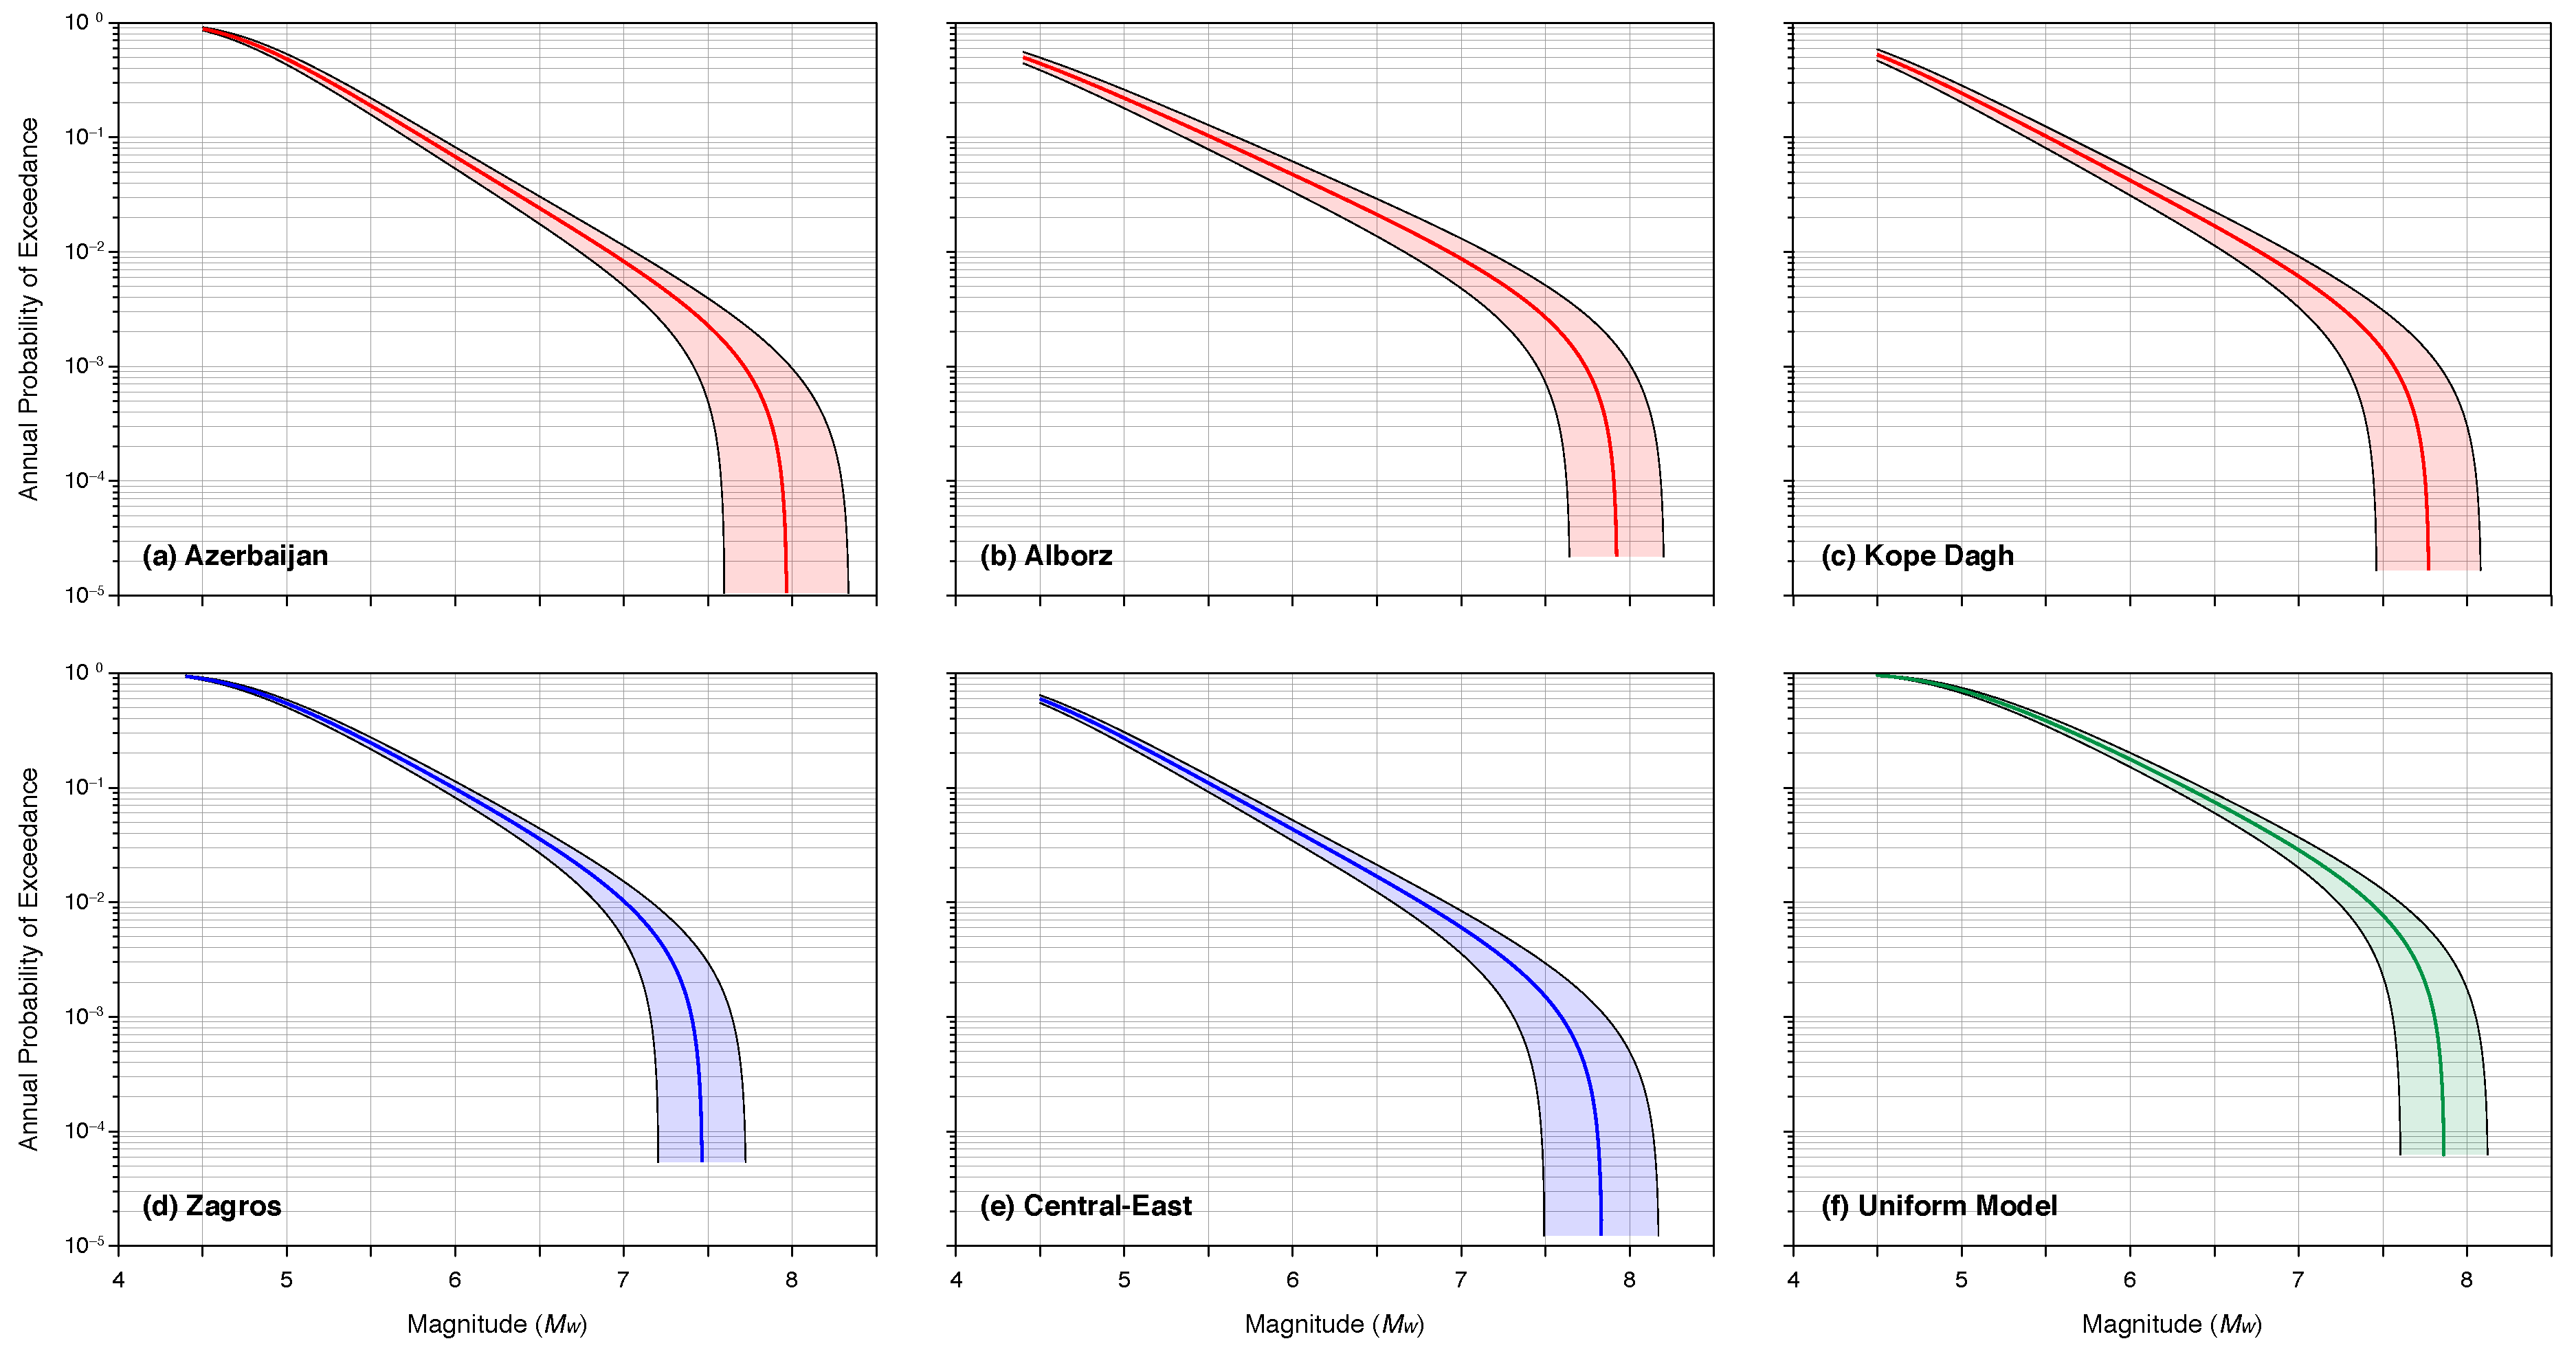
\includegraphics[width=\textwidth]{figures/pdf/figure-04} 
    \caption{Annual probability of exceedance as a function of earthquake magnitude for seismic tectonic regions of (a) Alborz, (b) Azerbaijan, (c) Central Iran, (d) Kopeh Dagh, (e) Uniform (f) Zagros. The shaded range indicates the models' $\pm 1$ standard deviation.}
    \label{fig:annualp}
\end{figure*}

\section{Seismicity Parameters}

Following the general approach described in the previous section and using the infrmation collected about the seismic catalog and its completeness, we computed the seismicity parameters $a$ and $b$, and the maximum magnitude $M_{\max}$ using the seismic hazard assessment software HA3 (version 3). This software implements the procedures developed by \citet{Kijko_1989_BSSA, Kijko_1992_BSSA}, and \citet{Kijko_2004_PAG}. HA3 is widely used for this type of computations and is regarded as a reliable tool in seismic hazard analysis \citep[see, for instance,][]{}\textcolor{red}{[references needed]}.

As mentioned before, the $a$-value is estimated based on the smoothed number of events ($M \geq 3$) per grid cell, and thus is variable throughout our region of interest. On the other hand, we consider the $b$-value and $M_{\max}$ to be constant within a given seismic zone. In this study we compute values for two different models. In the first model we obtain these parameters independently for each one of the seismic zones influencing the seismic hazard of northern Iran. That means we obtain distinct values of $b$ and $M_{\max}$ for Azerbaijan, Alborz, and Kopeh Dagh, which are our main seismic zones in northern Iran, as well as for the portions of the Zagros and Central-East seismic zones within our region of interest (see Fig.~\ref{fig:iran} for reference). In the second model we consider the whole region of interest as a uniform seismic zone. Admittedly, the second model is somewhat unrealistic if considered from the point of view that different seismic zones have different seismicity parameters. We thought, however, that computing results for a uniform model was useful for the analysis of results and comparisons with other studies.

Table \ref{tab:params} shows the parameters $b$ and $M_{\max}$ obtained using HA3 for the five seismic zones in our region of interest and for the uniform regional model, along with the observed maximum magnitude, $M_{\max}^{\mathrm{obs}}$. Fig.~\ref{fig:annualp} shows the obtained annual probability of exceedance as a function of earthquake magnitude.

% *********************************************************************************************************************
% OLD
% *********************************************************************************************************************

% For each of the three seismic regions, Gutenberg-Richter parameters and maximum magnitude ($M_{max}$) were calculated using Seismic Hazard Assessment code (HA3) \citep{kijko2004}. The regional maximum magnitude for each region is estimated by the \citet{Kijko1989} method, which is implemented in the HA3 package. For smoothed seismicity areas, $b-value$ is assumed constant. The $a-value$ can vary spatially and is determined by counting earthquakes above $M$ 3.0 in each grid cells.

% \citet{Karimiparidari2013} applied the Maximum Curvature (MAXC) technique \citep{Wyss1999, Wiemer2000} by ZMap \citep{Wiemer2001} to calculate the level of completeness of instrumental part of the catalog.  Following the \citet{Karimiparidari2013}, we assume the catalog is complete for earthquakes with magnitude 4.5, 4.4, 4.5, 4.5, and 4.4 for Azerbaijan, Alborz,  Kopeh-Dagh, Central Iran, and Zagros tectonic seismic regions, respectively. For the uniform model we used 4.5 as a completeness magnitude. In this study we use those magnitudes of completeness as the magnitude threshold in the calculation of the seismicity parameters. We also used the seismicity parameters of \citet{Karimiparidari2013} as the priory information in HA3 code. The updated values are displayed in Table \ref{tab:b_value}.  Annual occurrence rate of the earthquake for each region is shown in Fig.~\ref{fig:annual_m}.

% *********************************************************************************************************************
% OLDER
% *********************************************************************************************************************

% For each of the three seismic regions, Gutenberg-Richter parameters and Max magnitude ($M_{max}$) were calculated using Seismic Hazard Assessment code (HA3) \citep{kijko2004}. The regional maximum magnitude for each region is estimated by the \citet{Kijko1989} method, which is implemented in the HA3 package. For smoothed seismicity areas, $b-value$ is assumed constant. The $a-value$ can vary spatially and is determined by counting earthquakes above $M$ 3.0 in grid cells.\\

% \citet{Karimiparidari2013} applied the Maximum Curvature (MAXC) technique \citep{Wyss1999, Wiemer2000} by ZMap \citep{Wiemer2001} to calculate the level of completeness of instrumental part of the catalog. In this study we use those magnitudes of completeness as the magnitude threshold in the calculation of the seismicity parameters. We also used the seismicity parameters of this study \citep{Karimiparidari2013} as the priory information in HA3 code. The updated values are displayed in Table 2.

% Following the \citet{Karimiparidari2013}, we assume the catalog is complete for earthquakes with magnitude 4.5, 4.4, and 4.5 for Azerbaijan, Alborz and Kopeh-Dagh tectonic seismic regions, respectively. The completeness of each region can be seen easily from the scatter plot of completeness test. 
